\section{Data and calculations}
Collect here all the results obtained: photos, data tables and personal observations are all welcome. When the data are numerous, gather them in tables. The experimental data and the data processing can also be merged into a single narrative if that reads better.

Write every formula used for the calculations, explaining what it is for and giving the units of each quantity. There are two common layouts: write all the formulae first and then the calculations with your data, or write each formula immediately followed by its calculation. A table suits the second layout well.

\paragraph{First layout.}
The amount of substance is obtained from the molar concentration $c$ and the volume $V$ of the solution:
\begin{equation}
    n = c \cdot V
    \label{eq:moles} % the label lets you refer to the equation with \cref{eq:moles}
\end{equation}
where $n$ is in \unit{\mole}, $c$ in \unit{\mole\per\litre} and $V$ in \unit{\litre}. Applying \cref{eq:moles} to the data (the starred environment \texttt{equation*} suppresses the number):
\begin{equation*}
    n = \qty{0.5}{\mole\per\litre} \cdot \qty{25e-3}{\litre} = \qty{1.25e-2}{\mole}
\end{equation*}
The volume is divided by 1000 because it was measured in millilitres.

\paragraph{Second layout.}
\begin{center}
    \renewcommand{\arraystretch}{1.6} % more vertical space between rows
    \begin{tabular}{l c l}
        \toprule
        \textbf{Formula} &               & \textbf{Calculation}                                                                       \\
        \midrule
        $n = c \cdot V$  & $\rightarrow$ & $n = \qty{0.5}{\mole\per\litre} \cdot \qty{25e-3}{\litre} = \qty{1.25e-2}{\mole}$          \\
        $m = n \cdot M$  & $\rightarrow$ & $m = \qty{1.25e-2}{\mole} \cdot \qty{34.01}{\gram\per\mole} = \qty{0.425}{\gram}$          \\
        $c = m / V$      & $\rightarrow$ & $c = \qty{0.425}{\gram} / \qty{0.100}{\litre} = \qty{4.25}{\gram\per\litre}$               \\
        \bottomrule
    \end{tabular}
\end{center}

\subsection{Experimental data}
Report \emph{all} the experimental data, highlighting where necessary the outliers, that is the values rejected on the basis of a statistical test. Whenever possible, collect the data in tables; the \texttt{S} column type of \texttt{siunitx} aligns numbers on the decimal point (\cref{tab:data}).

\begin{table}[ht]
    \centering
    \begin{tabular}{c S[table-format=2.2] S[table-format=1.3]}
        \toprule
        {Trial} & {Volume [\unit{\milli\litre}]} & {Absorbance} \\
        \midrule
        1       & 10.05                          & 0.512        \\
        2       & 15.10                          & 0.768        \\
        3       & 20.00                          & 1.021        \\
        \bottomrule
    \end{tabular}
    \caption{Experimental data.}
    \label{tab:data}
\end{table}

\subsection{Data processing}
Report the calculations made from the experimental results, stating the mathematical relationships used. Processing may also include diagrams and plots, and sometimes the statistical treatment of the data. Plots are drawn with \texttt{pgfplots}, either from coordinates typed in the source (\cref{fig:solubility}) or from a data file (\cref{fig:kinetics}).

\begin{figure}[ht]
    \centering
    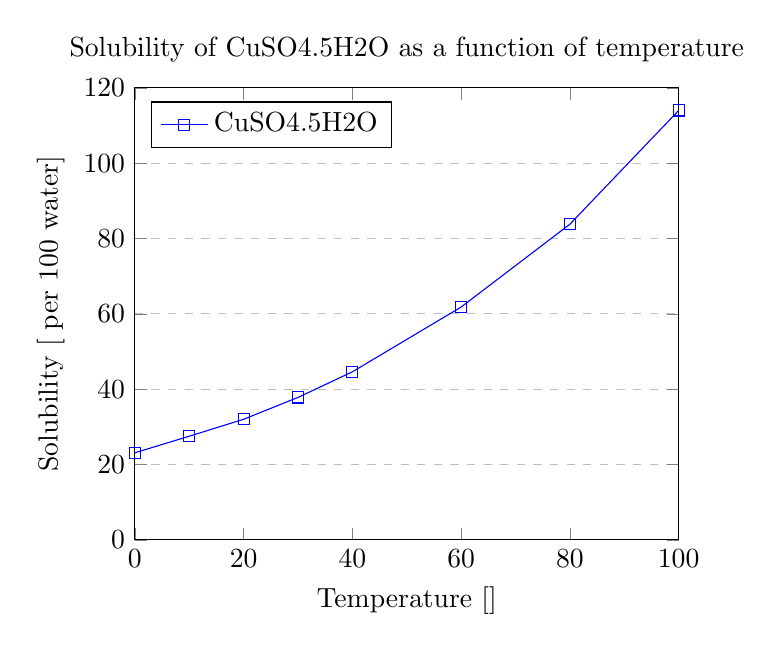
\begin{tikzpicture}
        \begin{axis}[
                width=0.7\textwidth,
                title={Solubility of \ce{CuSO4.5H2O} as a function of temperature},
                xlabel={Temperature [\unit{\degreeCelsius}]},
                ylabel={Solubility [\unit{\gram} per \qty{100}{\gram} water]},
                xmin=0, xmax=100,
                ymin=0, ymax=120,
                xtick={0,20,...,100},
                ytick={0,20,...,120},
                legend pos=north west,
                ymajorgrids=true,
                grid style=dashed,
            ]
            \addplot[color=blue, mark=square]
            coordinates {(0,23.1)(10,27.5)(20,32)(30,37.8)(40,44.6)(60,61.8)(80,83.8)(100,114)};
            \legend{\ce{CuSO4.5H2O}}
        \end{axis}
    \end{tikzpicture}
    \caption{Solubility of copper(II) sulfate pentahydrate in water as a function of temperature.}
    \label{fig:solubility}
\end{figure}

\begin{figure}[ht]
    \centering
    \begin{tikzpicture}
        \begin{axis}[
                width=0.7\textwidth,
                xlabel={Time [\unit{\minute}]},
                ylabel={Mole fraction},
                xmin=0, ymin=0, ymax=1,
                legend style={at={(0.97,0.5)}, anchor=east},
                grid=major,
                grid style=dashed,
            ]
            \addplot[color=red, mark=*, mark size=1.5pt] table {data/data.txt};
            \addplot[color=blue, mark=triangle*] table {data/data2.txt};
            \legend{\ce{A}, \ce{B}}
        \end{axis}
    \end{tikzpicture}
    \caption{Reaction \ce{A -> B}: mole fractions read from \texttt{data/data.txt} and \texttt{data/data2.txt}.}
    \label{fig:kinetics}
\end{figure}
